% TOMWare.M — Reviewer 3 COMPLETE Overleaf snippets
% Access-2026-38745 (minor points; reuses R1/R2 evidence)

% === R3-1 AntiDebug matched (reuse) ===
% 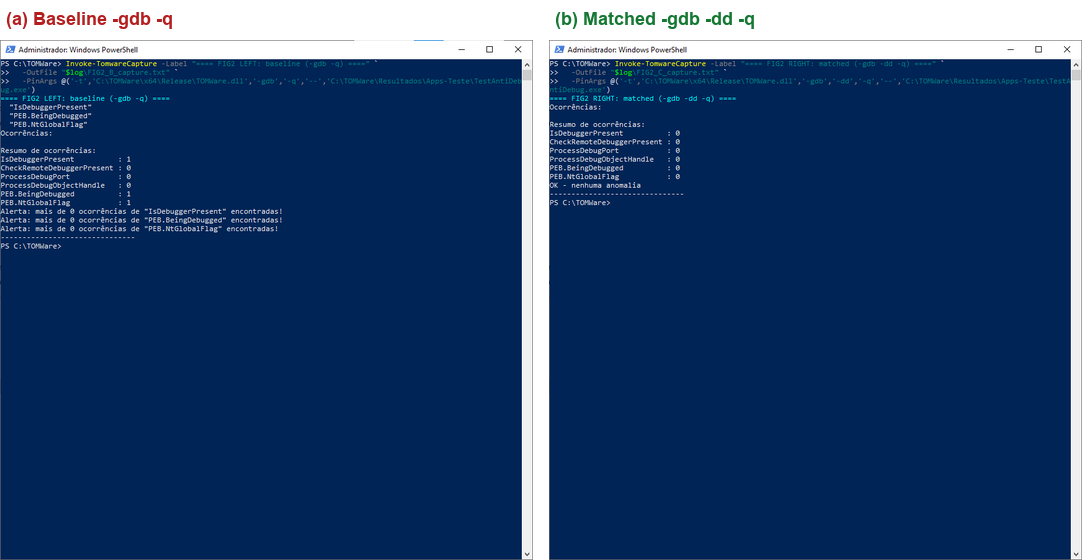
\includegraphics[width=\textwidth]{fig_antidebug_matched.png}
% Baseline: -gdb -q ; Treatment: -gdb -dd -q (Reviewer typo -gbd = -gdb).

% === R3-2 Re-execution rate / selection bias ===
Earlier corpus timing reports allowed additional attempts after a failed first run.
Under a fixed-1-attempt reading of those reports, 22/31 samples
(71.0\%) completed on the first attempt, whereas 9/31
(29.0\%) required at least one re-execution. Retaining only eventually
successful trials can inflate apparent success and bias timing summaries toward
threshold-satisfying runs. We therefore (i) report the first-attempt recount
explicitly, (ii) treat corpus aggregates as descriptive, and (iii) redesign the
SkewMask oracle to a fixed-N protocol that retains every run.

% === R3-3 Uncertainty / descriptive claims ===
% Oracle fixed-N=30 (all retained): B above 23/30,
% median 3213.49, IQR [3062.36, 3511.81],
% 95\% bootstrap CI [3140.16, 3432.05];
% C OK 30/30, median 2114.34,
% IQR [2109.25, 2122.07],
% 95\% CI [2112.96, 2119.14].
% Corpus PE-level medians remain descriptive summaries (no significance tests).

% === R3-4 Related systems table ===
% Prefer tab:related-r3 / corpus comparison already prepared for R2.
\begin{table}[!t]
\centering
\caption{Concise architectural comparison with closely related systems.
No shared-workload empirical head-to-head was performed in this revision.}
\label{tab:related-r3}
\begin{tabular}{p{2.2cm} p{2.6cm} p{2.6cm} p{2.6cm} p{3.2cm}}
\hline
Dimension & Arancino & COBAI & Peekaboo & TOMWare.M \\
\hline
Role & Defensive Pin layer & DBI defense tooling & Transparent analysis / DBI evasion handling & Modular defensive Pintool (Win x64) \\
Activation & Integrated layer & Framework-specific & Framework-specific & Selective knobs (-dd/-dp/-de/-dm/-do, -da) \\
Eval. here & Not re-run & Not re-run & Not re-run & Matched oracles + compatibility probe \\
Empirical H2H & No & No & No & --- \\
\hline
\end{tabular}
\end{table}

In our comparison, TOMWare.M combines selective module activation with matched
oracle validation and an auditable compatibility-probe protocol under Intel Pin
on Windows x64.

% === R3-5 Language / formatting checklist ===
% - Unify hyphenation of anti-instrumentation / anti-debug.
% - Fix Reviewer typo mapping: -gbd -> -gdb in text/captions.
% - Consistent spaces around math/knobs (-gdb -dd).
% - Table/figure caption punctuation and non-breaking spaces for units.
% - PURGE manuscript-wide: "unvalidated" / "inconclusive" for AntiDebug.
% - Do NOT claim empirical superiority vs Arancino/COBAI/Peekaboo.
